

% l = 8
\begin{figure}[H]
\begin{center}
\subfloat{
\resizebox{8cm}{5cm}{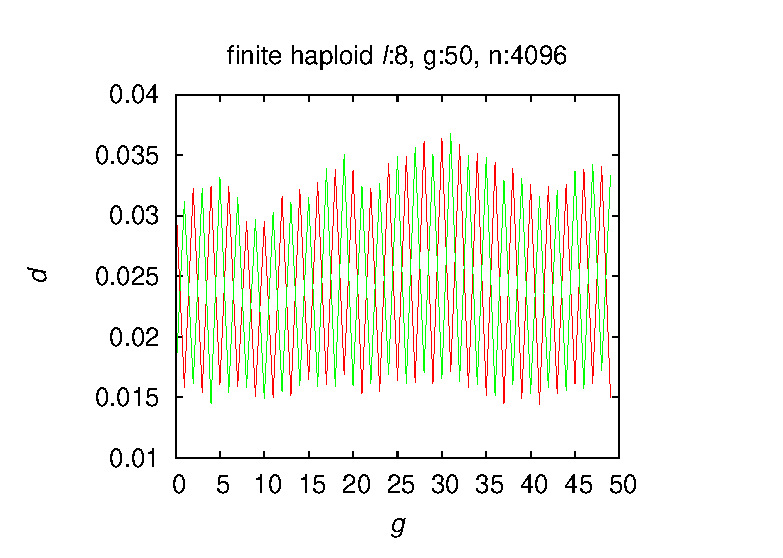
\includegraphics{figures/eps/osc/b8/n004096_osc_fin_hap.eps}}} \hspace{-3em}% 
\subfloat{
\resizebox{8cm}{5cm}{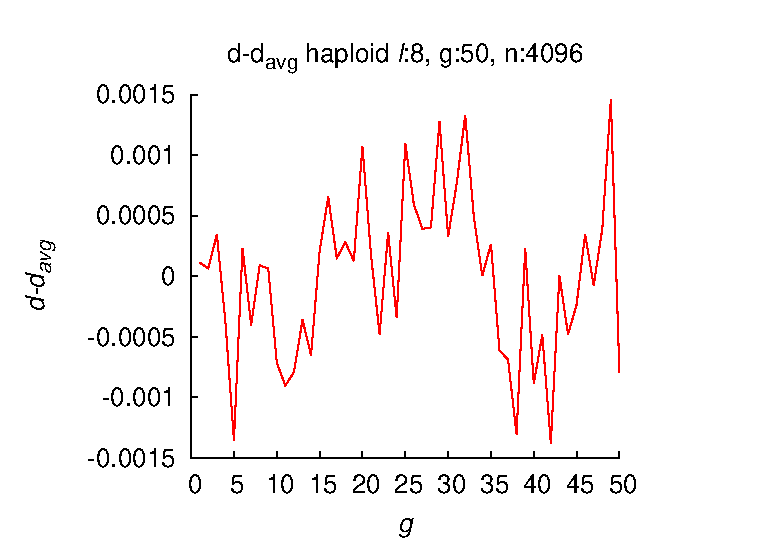
\includegraphics{figures/eps/osc/b8/n004096_osc_fin_hap_dist.eps}}} \vspace{-1em}  \hspace{-3em}% 

\end{center}
\begin{center}
\subfloat{
\resizebox{8cm}{5cm}{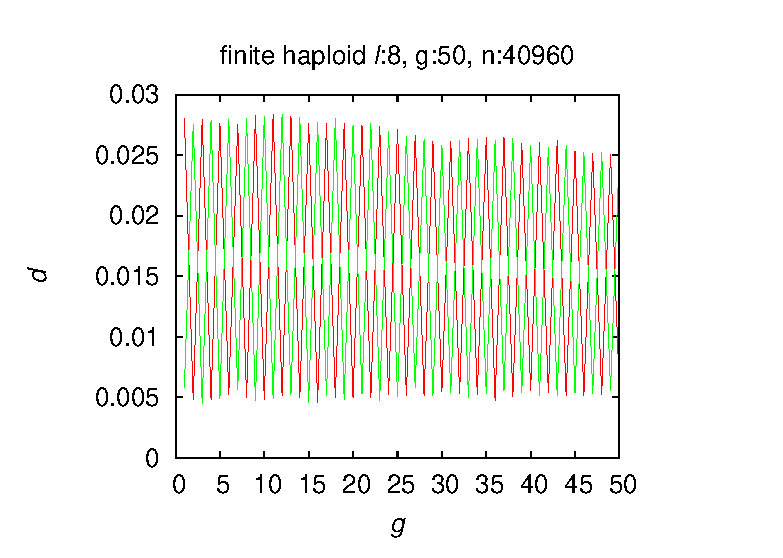
\includegraphics{figures/eps/osc/b8/n040960_osc_fin_hap.eps}}} \hspace{-3em}% 
\subfloat{
\resizebox{8cm}{5cm}{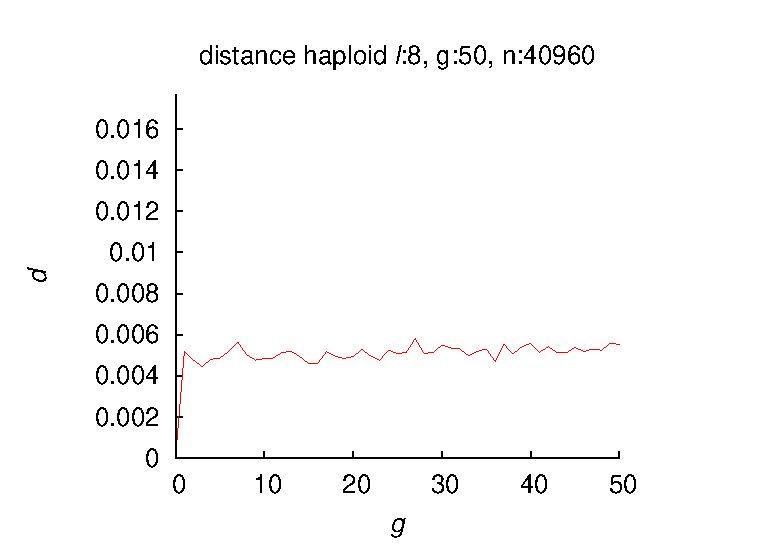
\includegraphics{figures/eps/osc/b8/n040960_osc_fin_hap_dist.eps}}} \vspace{-1em}  \hspace{-3em}% 
\end{center}

\begin{center}
\subfloat{
\resizebox{8cm}{5cm}{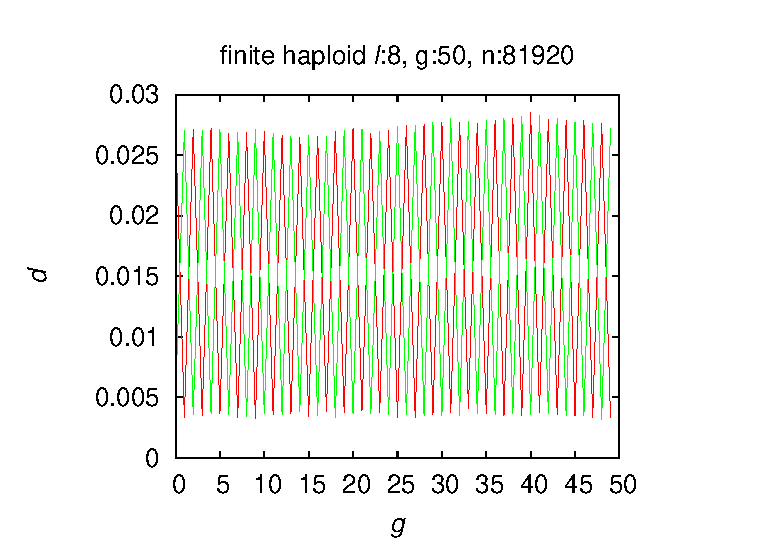
\includegraphics{figures/eps/osc/b8/n081920_osc_fin_hap.eps}}} \hspace{-3em}% 
\subfloat{
\resizebox{8cm}{5cm}{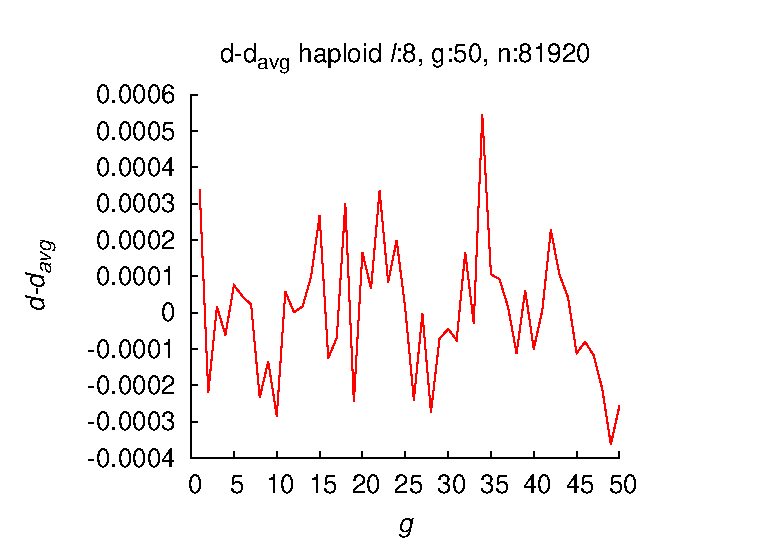
\includegraphics{figures/eps/osc/b8/n081920_osc_fin_hap_dist.eps}}} \vspace{-1em}  \hspace{-3em}% 
\end{center}


\begin{flushleft}
\subfloat{
\resizebox{8cm}{5cm}{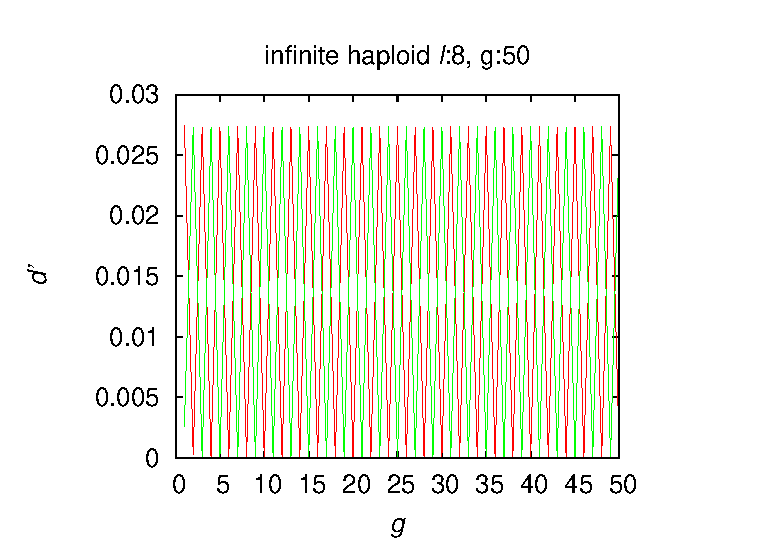
\includegraphics{figures/eps/osc/b8/osc_inf_hap.eps}}} \vspace{-0.5em} \hspace{-3em}%


\caption{\textbf{Infinite and finite haploid population oscillation behavior for genome length $\ell = 8$ (bits):} $d$ is
  distance between infinite or finite population ${\bm q}^n$ and infinite
  population limits ${{\bm p}^\ast}$ and ${{\bm q}^{\ast}}$ for $g$ generations and finite population size $n$.}
\label{oscillation_8h}
\end{flushleft}
\end{figure}


\begin{figure}[H]

\begin{center}
\subfloat{
\resizebox{8cm}{5cm}{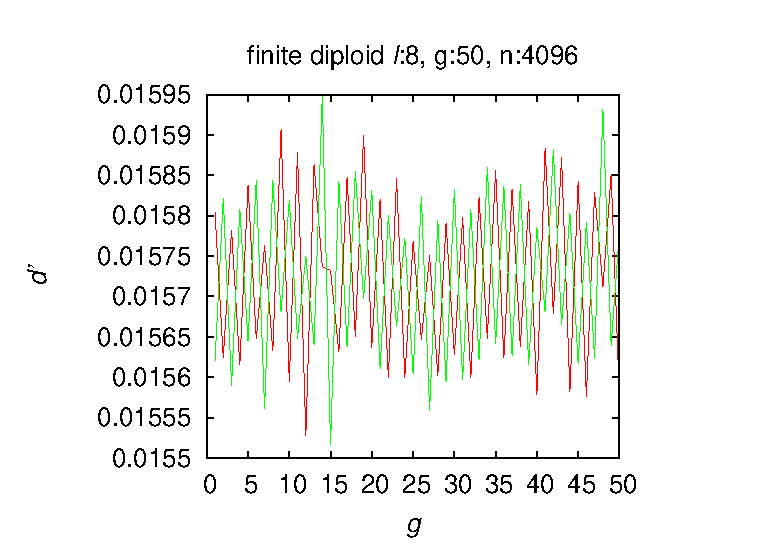
\includegraphics{figures/eps/osc/b8/n004096_osc_fin_dip.eps}}} \hspace{-3em}% 
\subfloat{
\resizebox{8cm}{5cm}{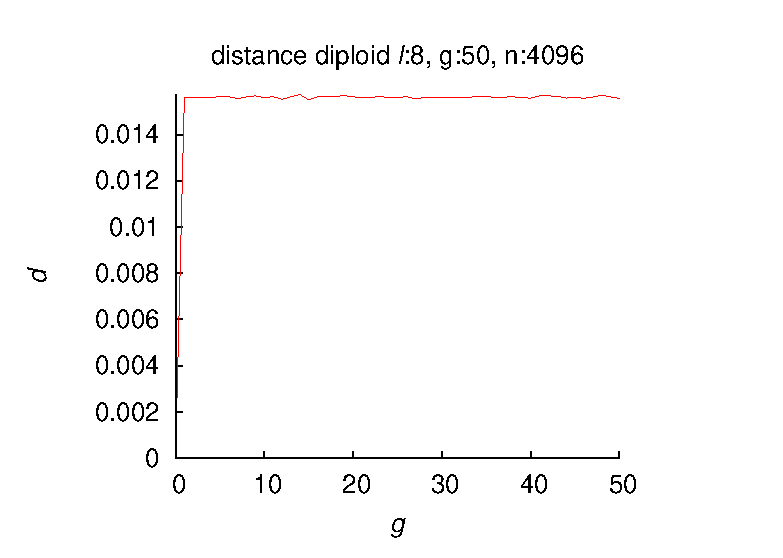
\includegraphics{figures/eps/osc/b8/n004096_osc_fin_dip_dist.eps}}}  \vspace{-1em}  \hspace{-3em}% 
\end{center}
\begin{center}
\subfloat{
\resizebox{8cm}{5cm}{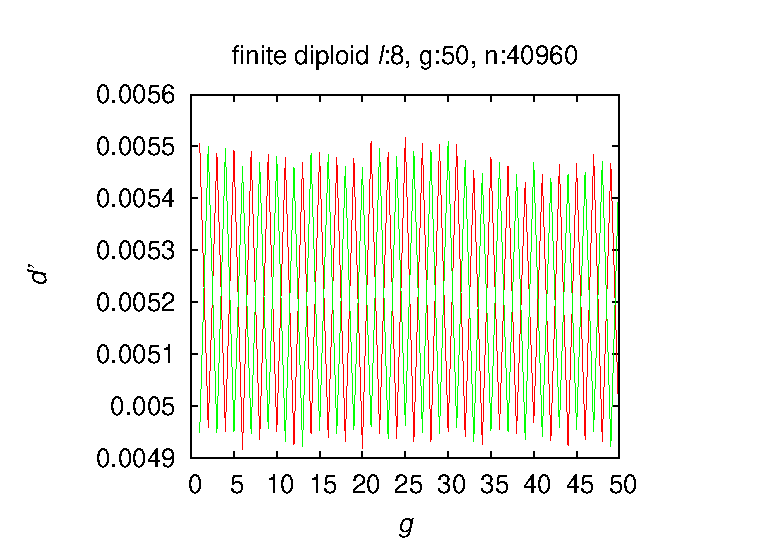
\includegraphics{figures/eps/osc/b8/n040960_osc_fin_dip.eps}}} \hspace{-3em}% 
\subfloat{
\resizebox{8cm}{5cm}{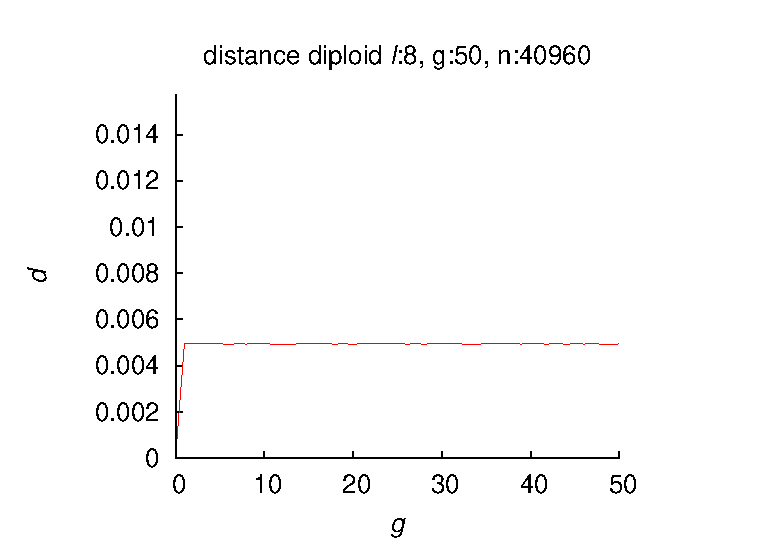
\includegraphics{figures/eps/osc/b8/n040960_osc_fin_dip_dist.eps}}}  \vspace{-1em}  \hspace{-3em}% 
\end{center}

\begin{center}
\subfloat{
\resizebox{8cm}{5cm}{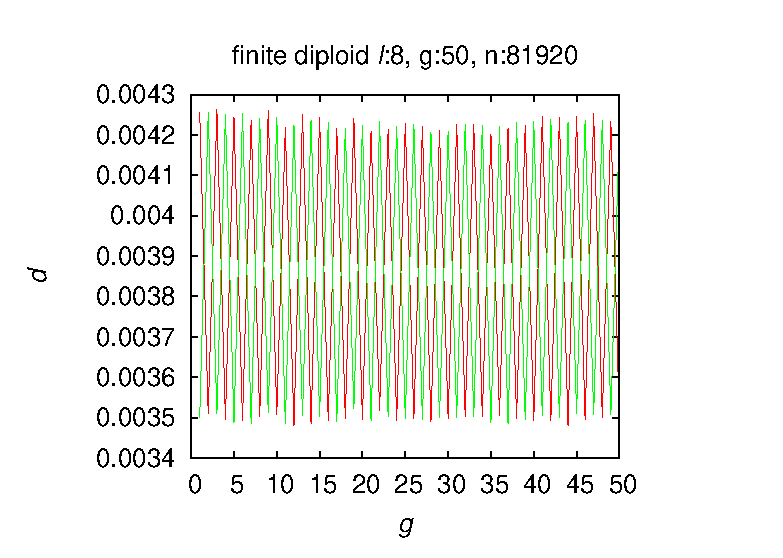
\includegraphics{figures/eps/osc/b8/n081920_osc_fin_dip.eps}}} \hspace{-3em}% 
\subfloat{
\resizebox{8cm}{5cm}{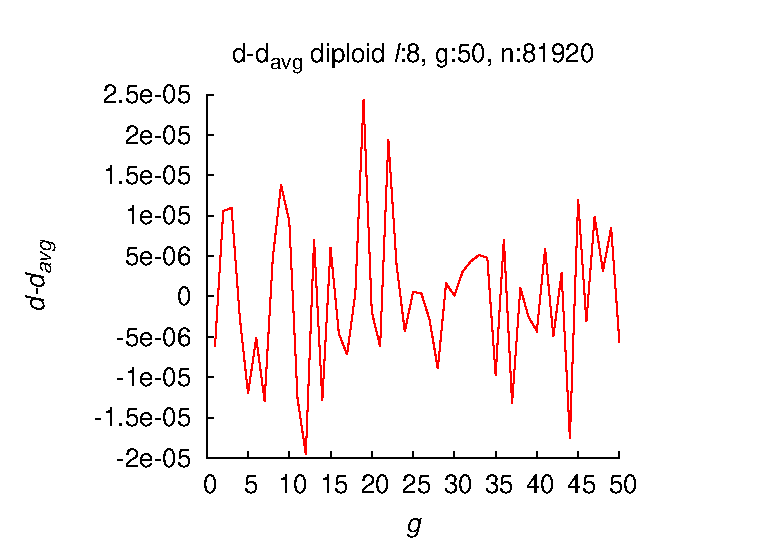
\includegraphics{figures/eps/osc/b8/n081920_osc_fin_dip_dist.eps}}}  \vspace{-1em}  \hspace{-3em}% 
\end{center}

\begin{flushleft}
\subfloat{
\resizebox{8cm}{5cm}{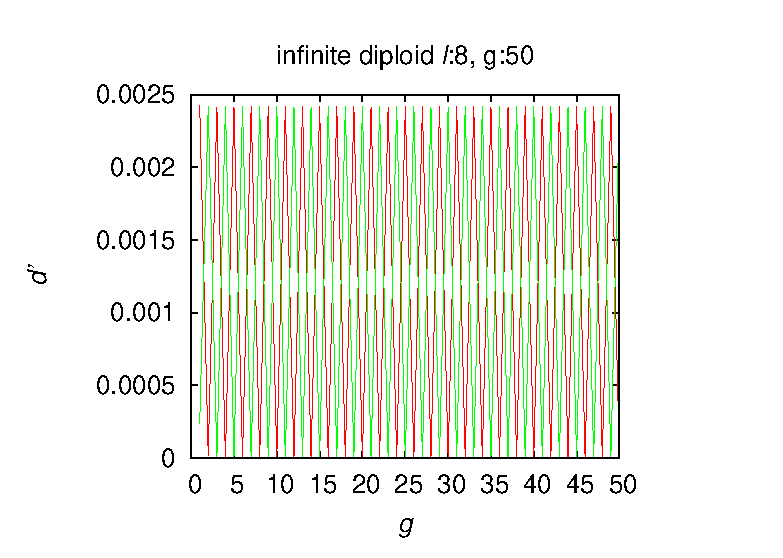
\includegraphics{figures/eps/osc/b8/osc_inf_dip.eps}}} \vspace{-0.5em} \hspace{-3em}%

\caption{\textbf{Infinite and finite diploid population oscillation behavior for genome length $\ell = 8$ (bits):} $d$ is
  distance between infinite or finite population ${\bm q}^n$ and infinite
  population limits ${{\bm p}^\ast}$ and ${{\bm q}^{\ast}}$ for $g$ generations and finite population size $n$.}
\label{oscillation_8d}
\end{flushleft}
\end{figure}

% l = 10

\begin{figure}[H]

\begin{center}
\subfloat{
\resizebox{8cm}{5cm}{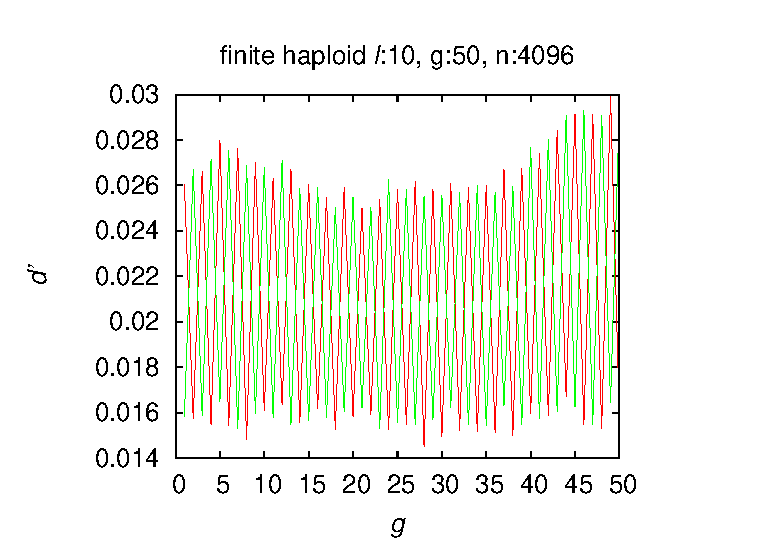
\includegraphics{figures/eps/osc/b10/n004096_osc_fin_hap.eps}}} \hspace{-3em}% 
\subfloat{
\resizebox{8cm}{5cm}{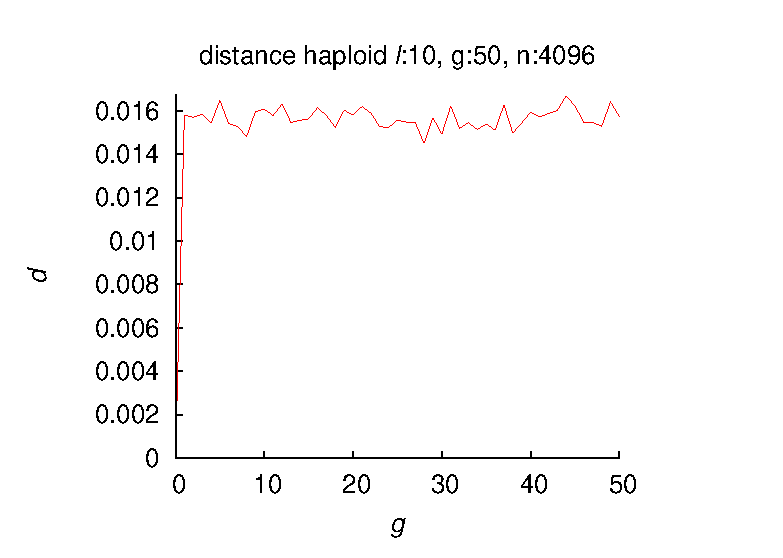
\includegraphics{figures/eps/osc/b10/n004096_osc_fin_hap_dist.eps}}} \vspace{-1em}  \hspace{-3em}% 
\end{center}
\begin{center}
\subfloat{
\resizebox{8cm}{5cm}{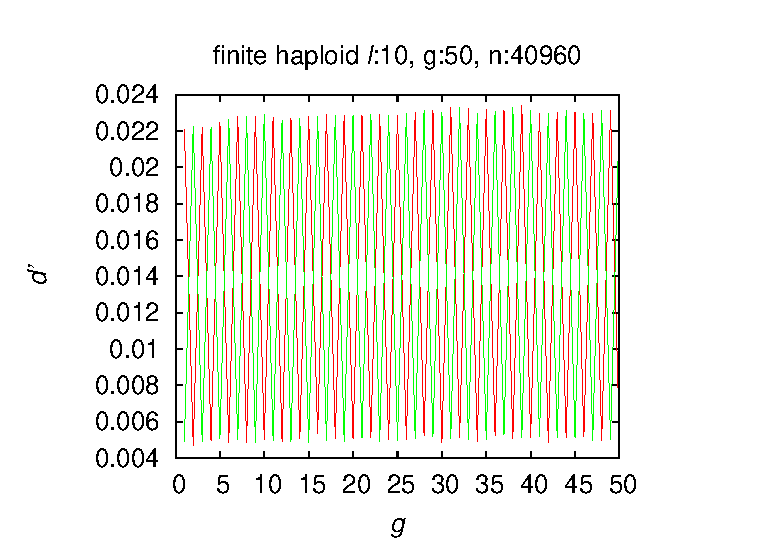
\includegraphics{figures/eps/osc/b10/n040960_osc_fin_hap.eps}}} \hspace{-3em}% 
\subfloat{
\resizebox{8cm}{5cm}{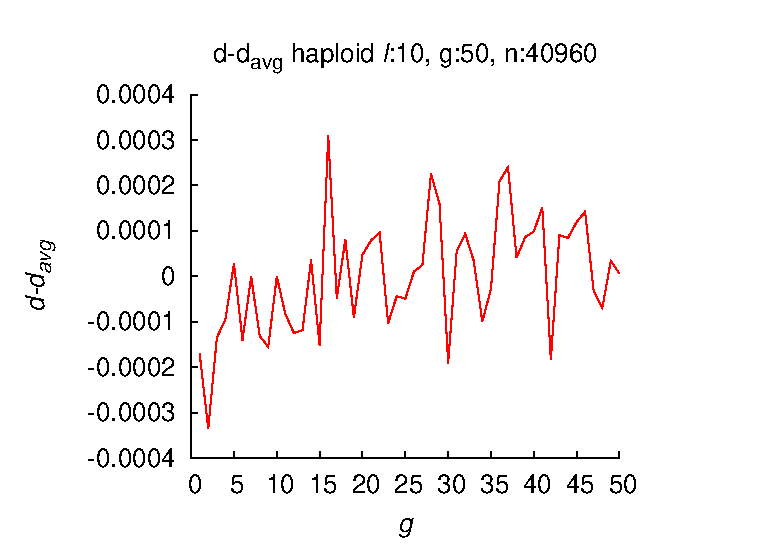
\includegraphics{figures/eps/osc/b10/n040960_osc_fin_hap_dist.eps}}} \vspace{-1em}  \hspace{-3em}% 
\end{center}

\begin{center}
\subfloat{
\resizebox{8cm}{5cm}{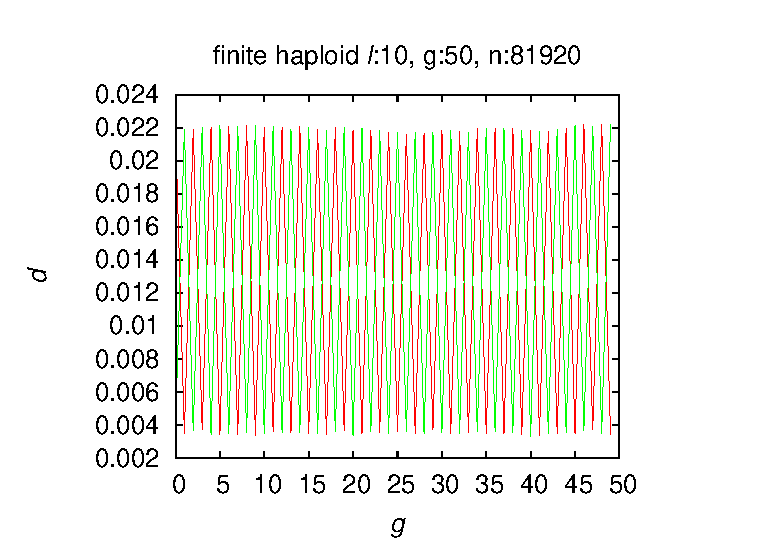
\includegraphics{figures/eps/osc/b10/n081920_osc_fin_hap.eps}}} \hspace{-3em}% 
\subfloat{
\resizebox{8cm}{5cm}{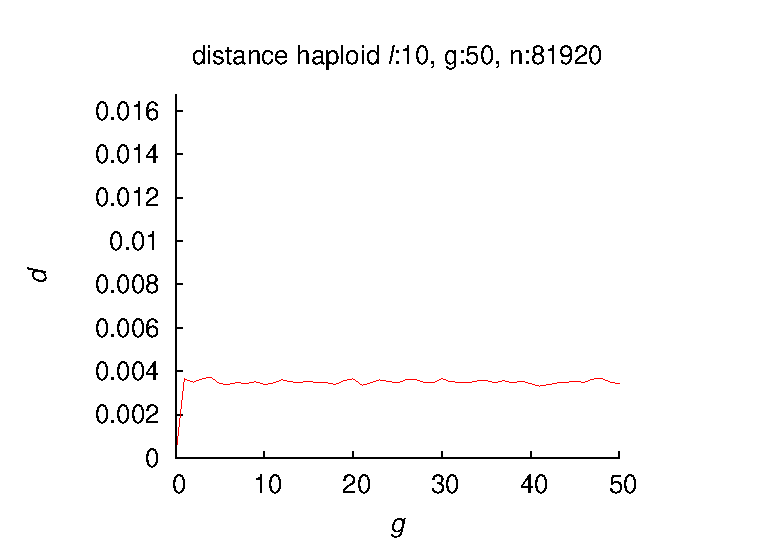
\includegraphics{figures/eps/osc/b10/n081920_osc_fin_hap_dist.eps}}} \vspace{-1em}  \hspace{-3em}% 
\end{center}

\begin{flushleft}
\subfloat{
\resizebox{8cm}{5cm}{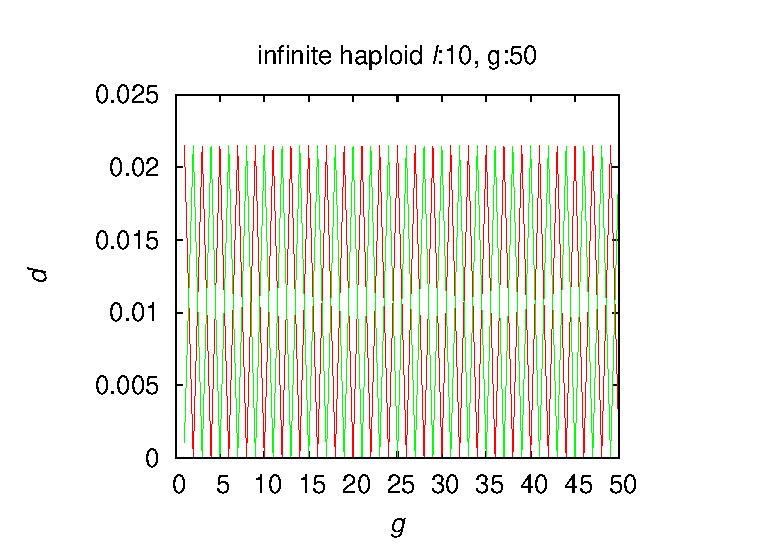
\includegraphics{figures/eps/osc/b10/osc_inf_hap.eps}}} \vspace{-0.5em} \hspace{-3em}%

\caption{\textbf{Infinite and finite haploid population oscillation behavior for genome length $\ell = 10$ (bits):} $d$ is
  distance between infinite or finite population ${\bm q}^n$ and infinite
  population limits ${{\bm p}^\ast}$ and ${{\bm q}^{\ast}}$ for $g$ generations and finite population size $n$.}
\label{oscillation_10h}
\end{flushleft}
\end{figure}


\begin{figure}[H]

\begin{center}
\subfloat{
\resizebox{8cm}{5cm}{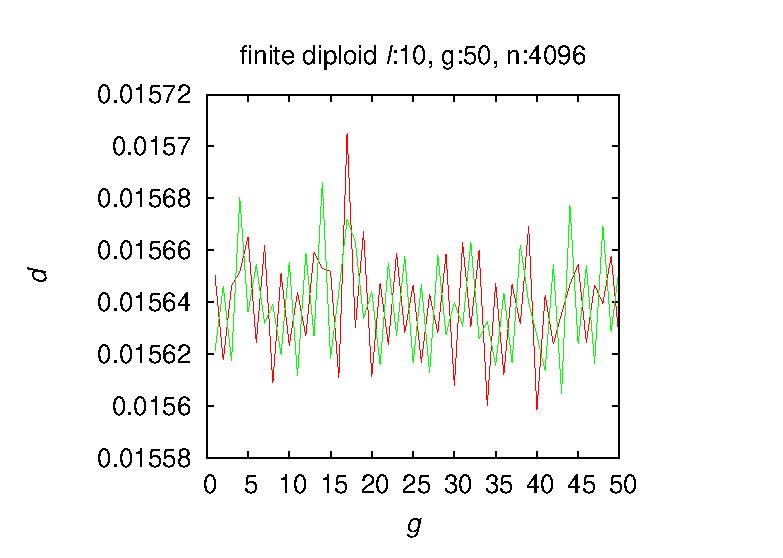
\includegraphics{figures/eps/osc/b10/n004096_osc_fin_dip.eps}}} \hspace{-3em}% 
\subfloat{
\resizebox{8cm}{5cm}{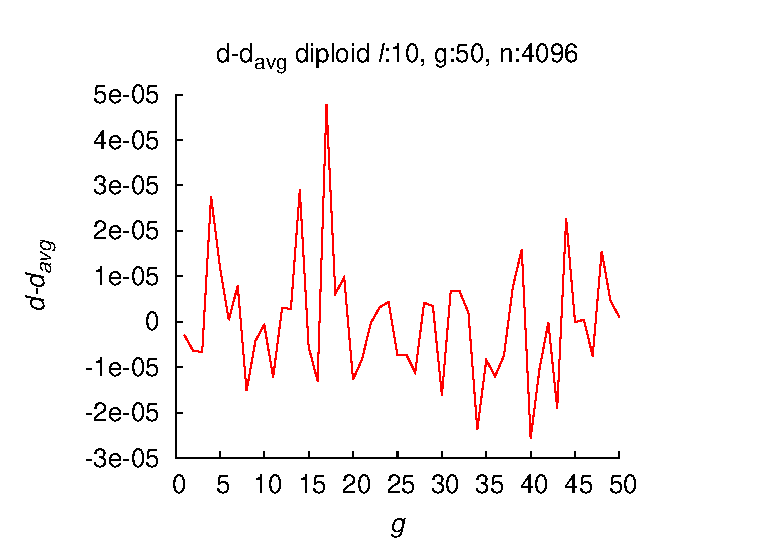
\includegraphics{figures/eps/osc/b10/n004096_osc_fin_dip_dist.eps}}}  \vspace{-1em}  \hspace{-3em}% 
\end{center}
\begin{center}
\subfloat{
\resizebox{8cm}{5cm}{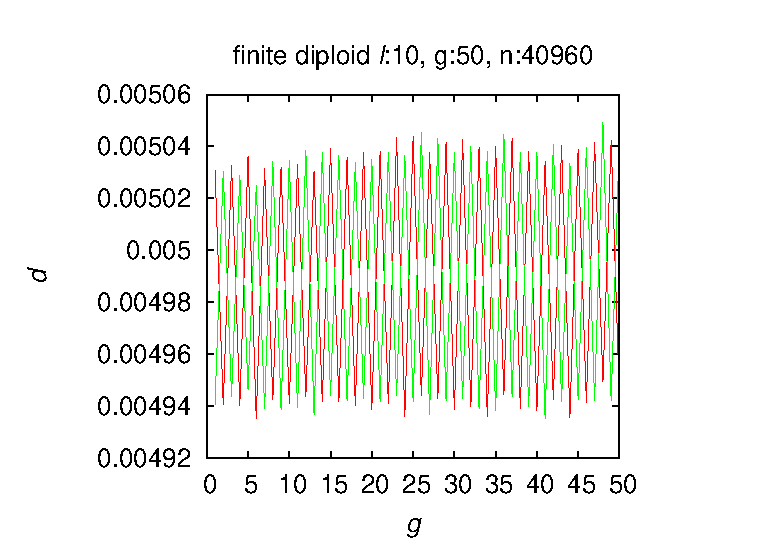
\includegraphics{figures/eps/osc/b10/n040960_osc_fin_dip.eps}}} \hspace{-3em}% 
\subfloat{
\resizebox{8cm}{5cm}{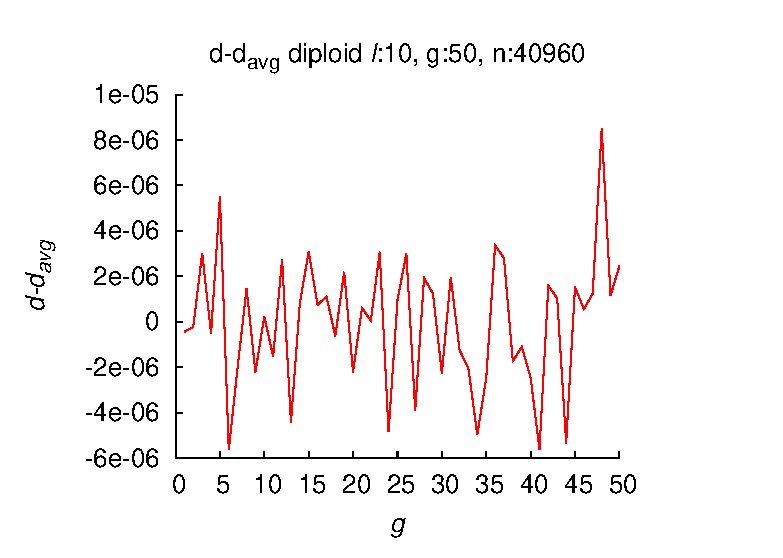
\includegraphics{figures/eps/osc/b10/n040960_osc_fin_dip_dist.eps}}}  \vspace{-1em}  \hspace{-3em}% 
\end{center}

\begin{center}
\subfloat{
\resizebox{8cm}{5cm}{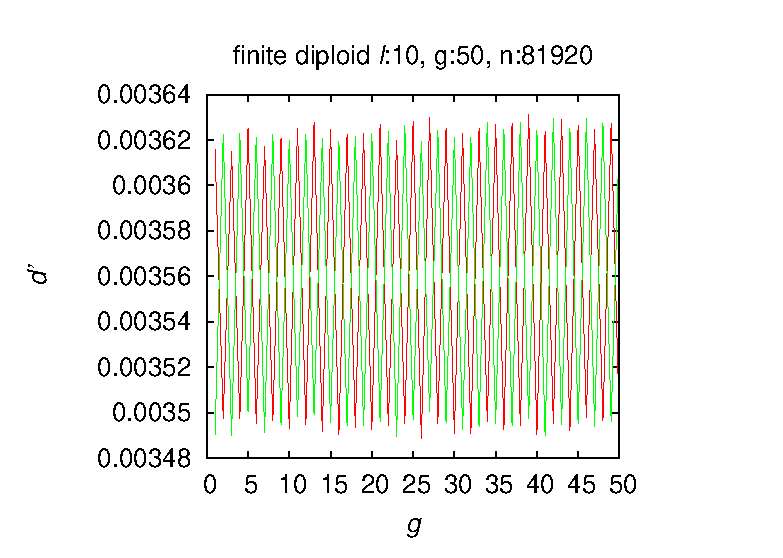
\includegraphics{figures/eps/osc/b10/n081920_osc_fin_dip.eps}}} \hspace{-3em}% 
\subfloat{
\resizebox{8cm}{5cm}{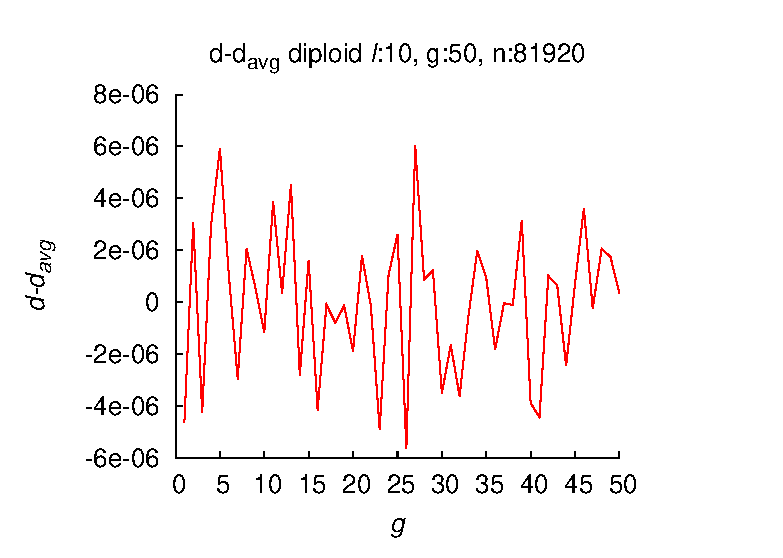
\includegraphics{figures/eps/osc/b10/n081920_osc_fin_dip_dist.eps}}}  \vspace{-1em}  \hspace{-3em}% 
\end{center}


\begin{flushleft}
\subfloat{
\resizebox{8cm}{5cm}{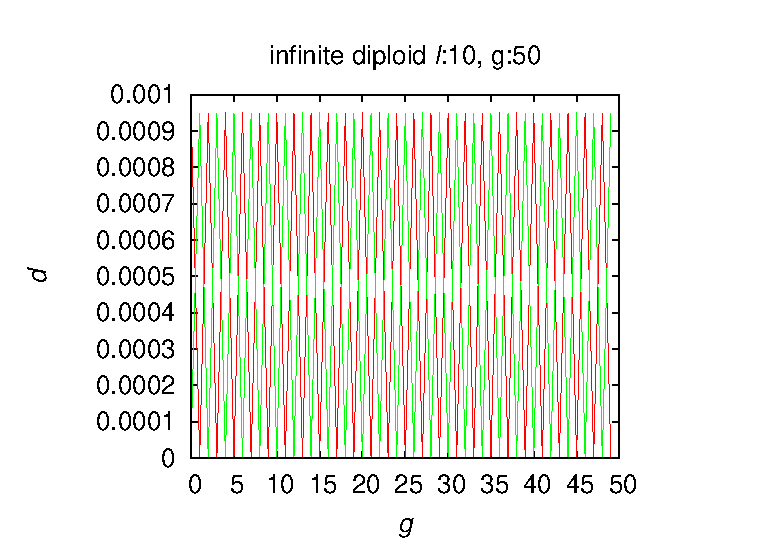
\includegraphics{figures/eps/osc/b10/osc_inf_dip.eps}}} \vspace{-0.5em} \hspace{-3em}%


\caption{\textbf{Infinite and finite population oscillation behavior for genome length $\ell = 10$ (bits):} $d$ is
  distance between infinite or finite population ${\bm q}^n$ and infinite
  population limits ${{\bm p}^\ast}$ and ${{\bm q}^{\ast}}$ for $g$ generations and finite population size $n$.}
\label{oscillation_10d}
\end{flushleft}
\end{figure}

% l = 12

\begin{figure}[H]

\begin{center}
\subfloat{
\resizebox{8cm}{5cm}{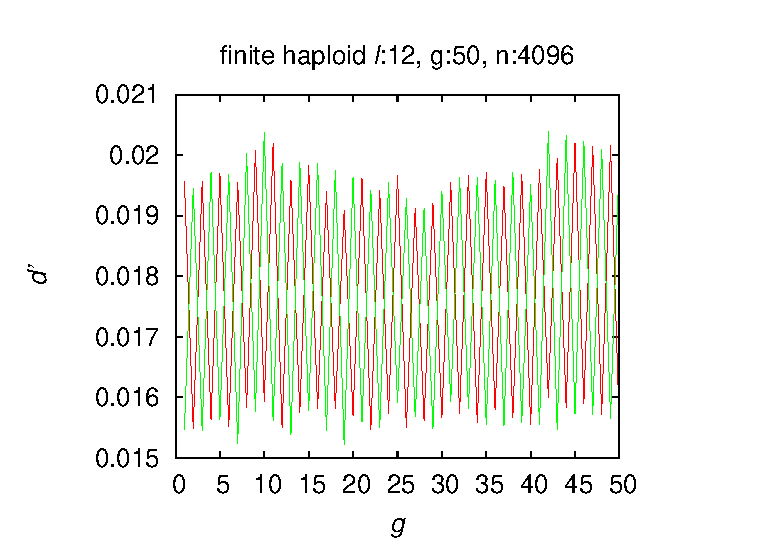
\includegraphics{figures/eps/osc/b12/n004096_osc_fin_hap.eps}}} \hspace{-3em}% 
\subfloat{
\resizebox{8cm}{5cm}{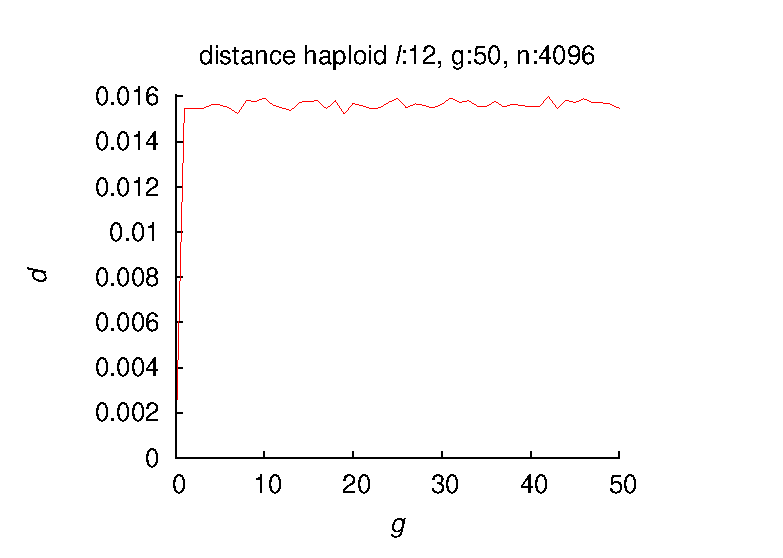
\includegraphics{figures/eps/osc/b12/n004096_osc_fin_hap_dist.eps}}} \vspace{-1em}  \hspace{-3em}% 
\end{center}
\begin{center}
\subfloat{
\resizebox{8cm}{5cm}{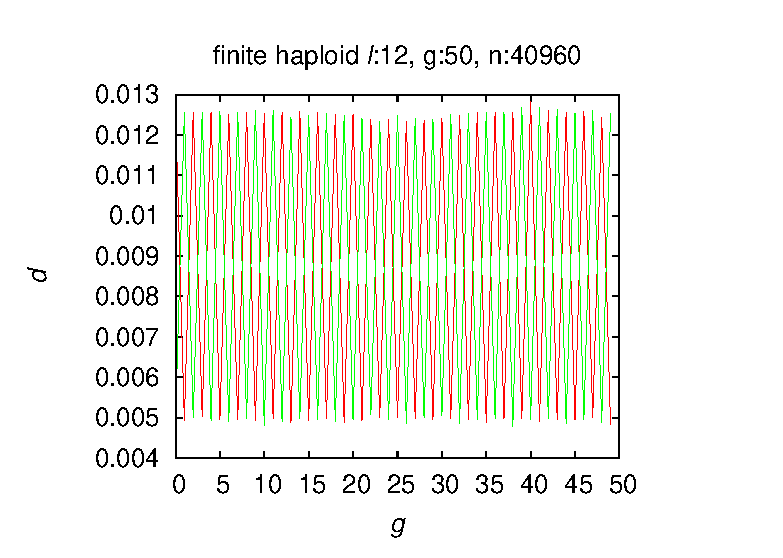
\includegraphics{figures/eps/osc/b12/n040960_osc_fin_hap.eps}}} \hspace{-3em}% 
\subfloat{
\resizebox{8cm}{5cm}{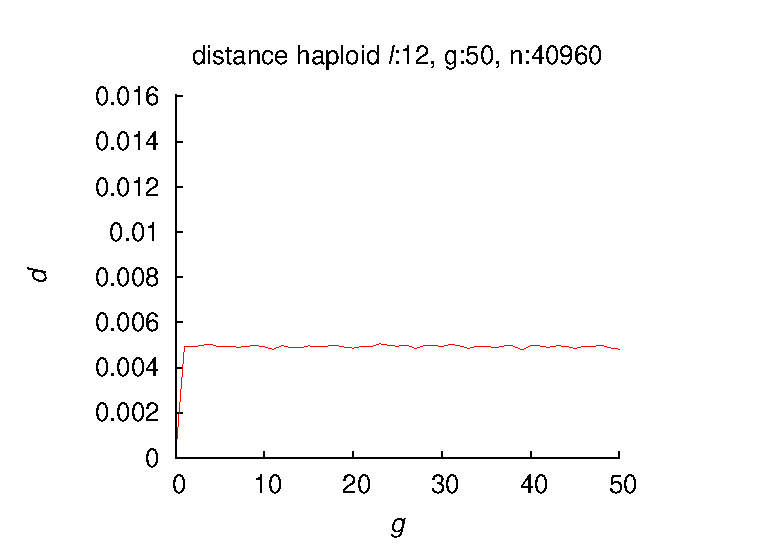
\includegraphics{figures/eps/osc/b12/n040960_osc_fin_hap_dist.eps}}} \vspace{-1em}  \hspace{-3em}% 
\end{center}
\begin{center}
\subfloat{
\resizebox{8cm}{5cm}{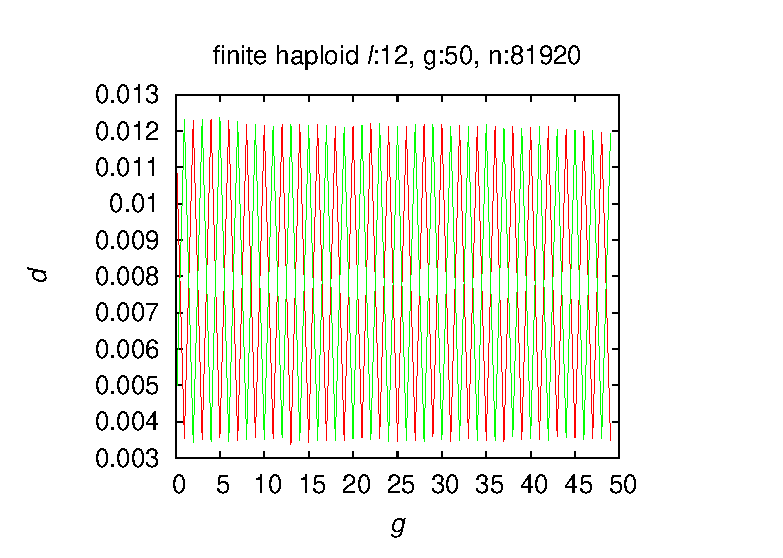
\includegraphics{figures/eps/osc/b12/n081920_osc_fin_hap.eps}}} \hspace{-3em}% 
\subfloat{
\resizebox{8cm}{5cm}{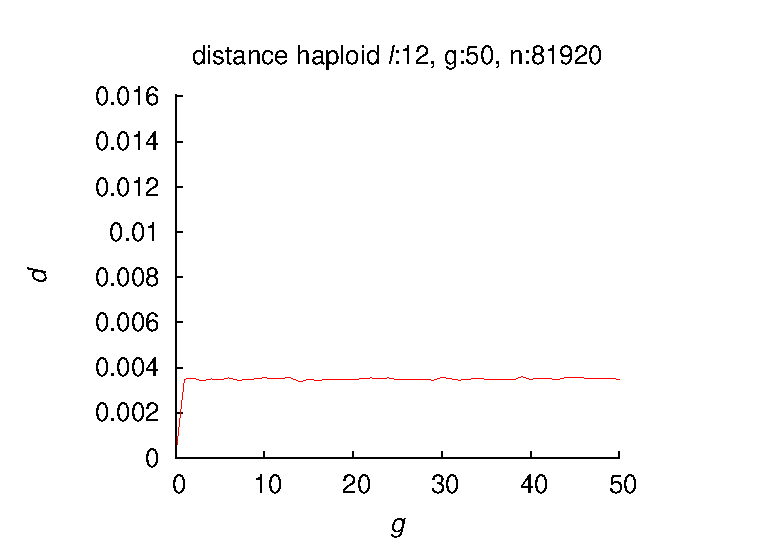
\includegraphics{figures/eps/osc/b12/n081920_osc_fin_hap_dist.eps}}} \vspace{-1em}  \hspace{-3em}% 
\end{center}

\begin{flushleft}
\subfloat{
\resizebox{8cm}{5cm}{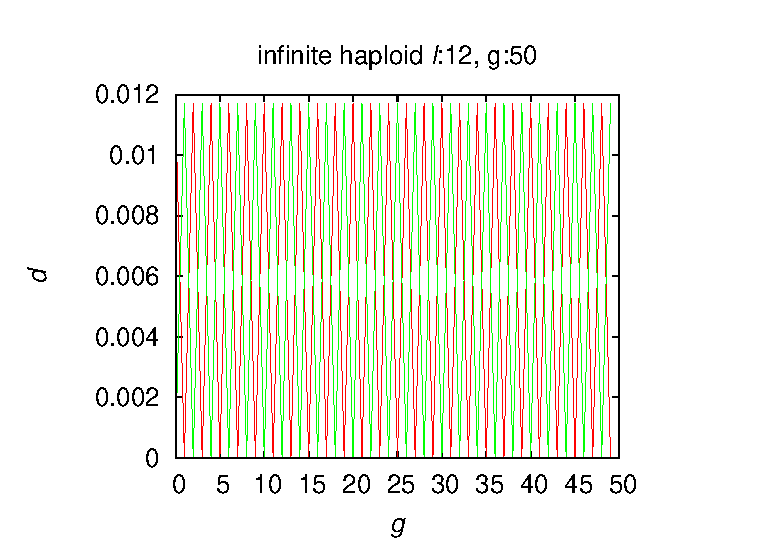
\includegraphics{figures/eps/osc/b12/osc_inf_hap.eps}}} \vspace{-0.5em} \hspace{-3em}%


\caption{\textbf{Infinite and finite haploid population oscillation behavior for genome length $\ell = 12$ (bits):} $d$ is
  distance between infinite or finite population ${\bm q}^n$ and infinite
  population limits ${{\bm p}^\ast}$ and ${{\bm q}^{\ast}}$ for $g$ generations and finite population size $n$.}
\label{oscillation_12h}
\end{flushleft}
\end{figure}

\begin{figure}[H]

\begin{center}
\subfloat{
\resizebox{8cm}{5cm}{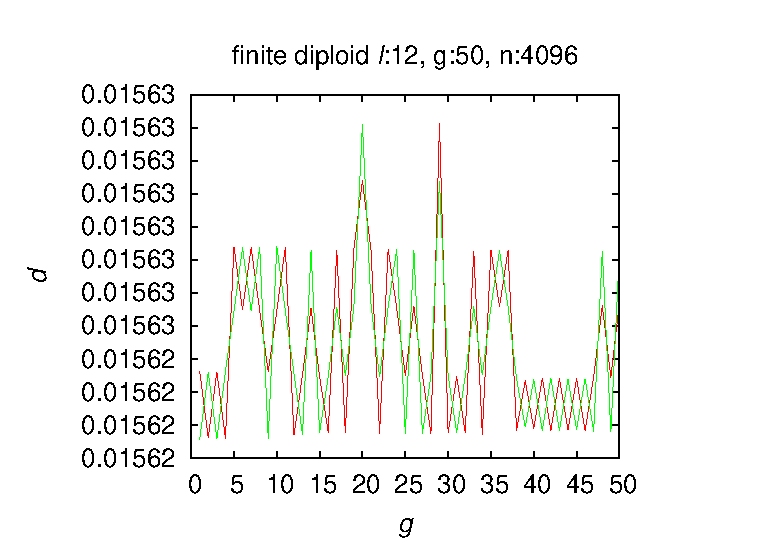
\includegraphics{figures/eps/osc/b12/n004096_osc_fin_dip.eps}}} \hspace{-3em}% 
\subfloat{
\resizebox{8cm}{5cm}{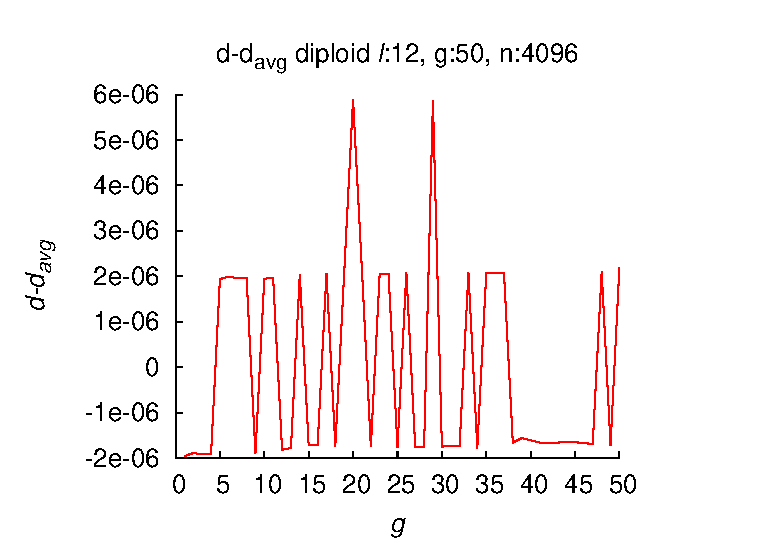
\includegraphics{figures/eps/osc/b12/n004096_osc_fin_dip_dist.eps}}}  \vspace{-1em}  \hspace{-3em}% 
\end{center}
\begin{center}
\subfloat{
\resizebox{8cm}{5cm}{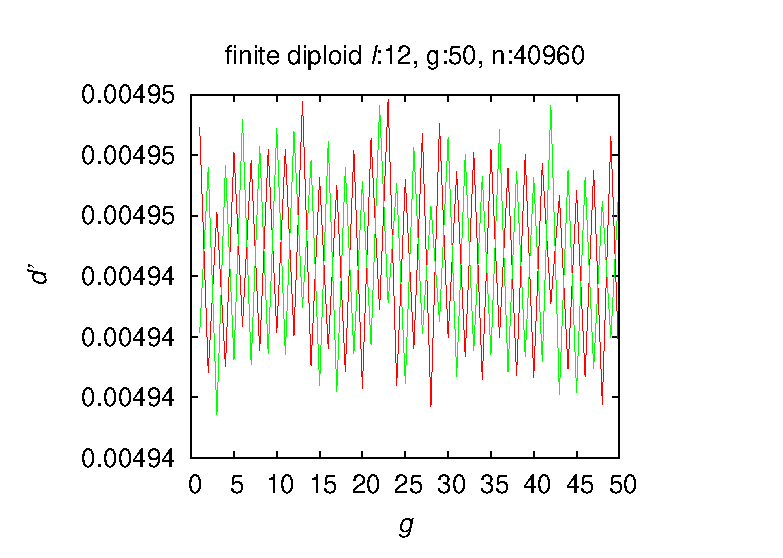
\includegraphics{figures/eps/osc/b12/n040960_osc_fin_dip.eps}}} \hspace{-3em}% 
\subfloat{
\resizebox{8cm}{5cm}{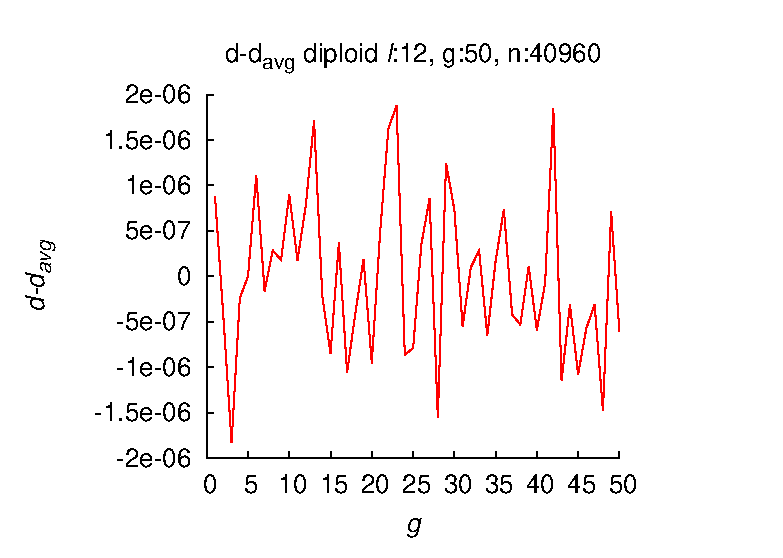
\includegraphics{figures/eps/osc/b12/n040960_osc_fin_dip_dist.eps}}}  \vspace{-1em}  \hspace{-3em}% 
\end{center}

\begin{center}
\subfloat{
\resizebox{8cm}{5cm}{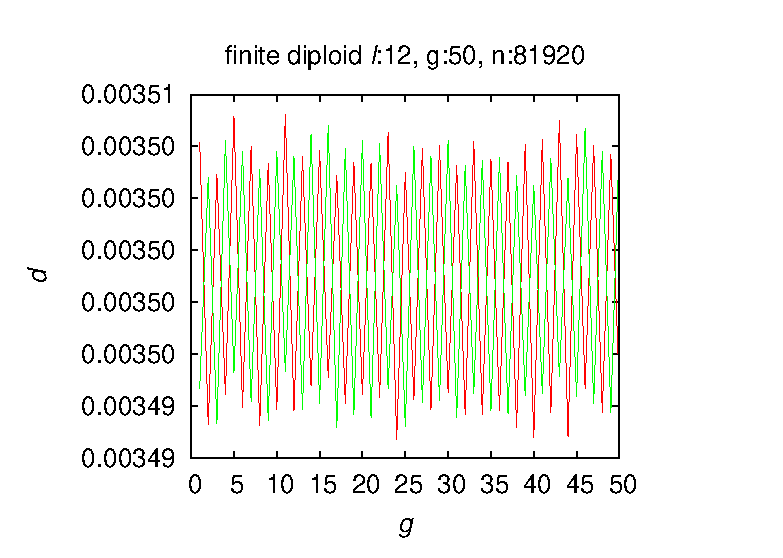
\includegraphics{figures/eps/osc/b12/n081920_osc_fin_dip.eps}}} \hspace{-3em}% 
\subfloat{
\resizebox{8cm}{5cm}{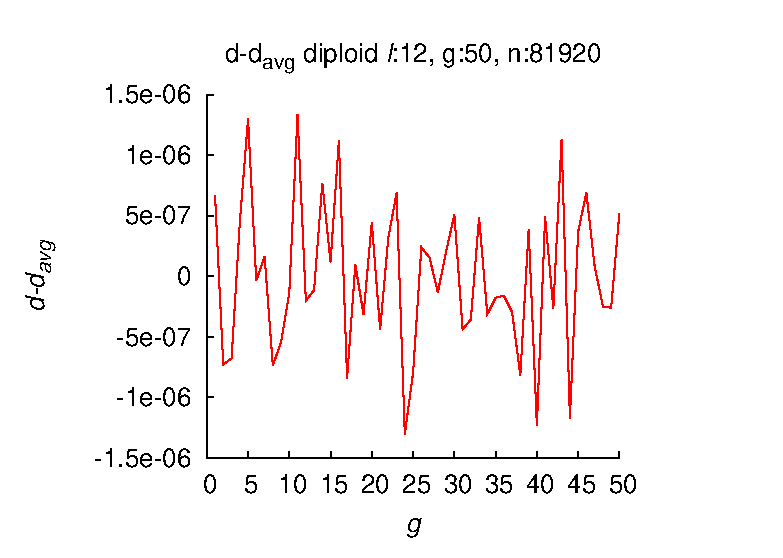
\includegraphics{figures/eps/osc/b12/n081920_osc_fin_dip_dist.eps}}}  \vspace{-1em}  \hspace{-3em}% 
\end{center}

\begin{flushleft}
\subfloat{
\resizebox{8cm}{5cm}{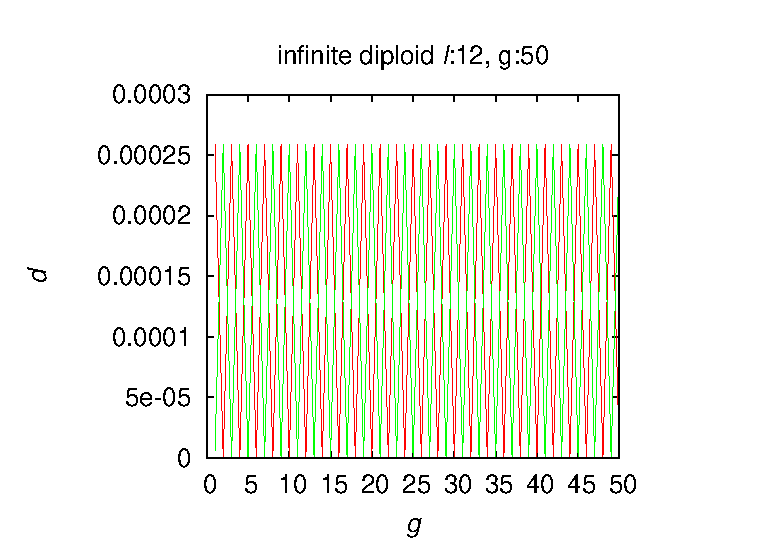
\includegraphics{figures/eps/osc/b12/osc_inf_dip.eps}}} \vspace{-0.5em} \hspace{-3em}%


\caption{\textbf{Infinite and finite diploid population oscillation behavior for genome length $\ell = 12$ (bits):} $d$ is
  distance between infinite or finite population ${\bm q}^n$ and infinite
  population limits ${{\bm p}^\ast}$ and ${{\bm q}^{\ast}}$ for $g$ generations and finite population size $n$.}
\label{oscillation_12d}
\end{flushleft}
\end{figure}


% l= 14


\begin{figure}[H]

\begin{center}
\subfloat{
\resizebox{8cm}{5cm}{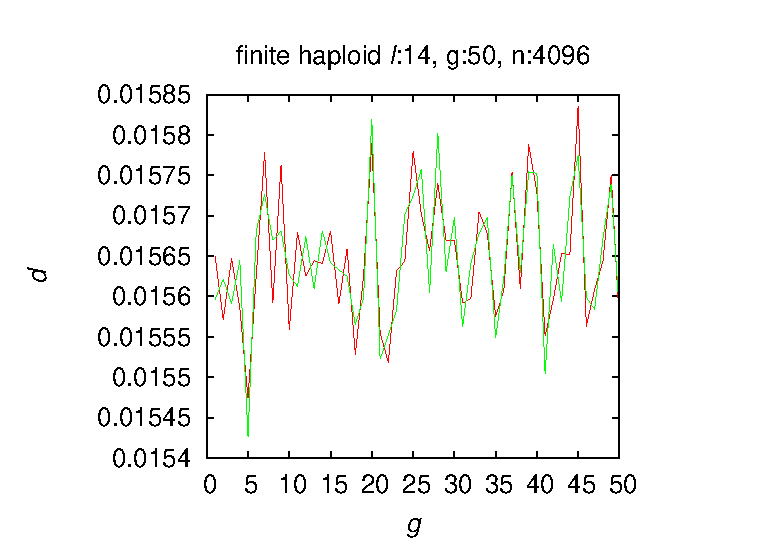
\includegraphics{figures/eps/osc/b14/n004096_osc_fin_hap.eps}}} \hspace{-3em}% 
\subfloat{
\resizebox{8cm}{5cm}{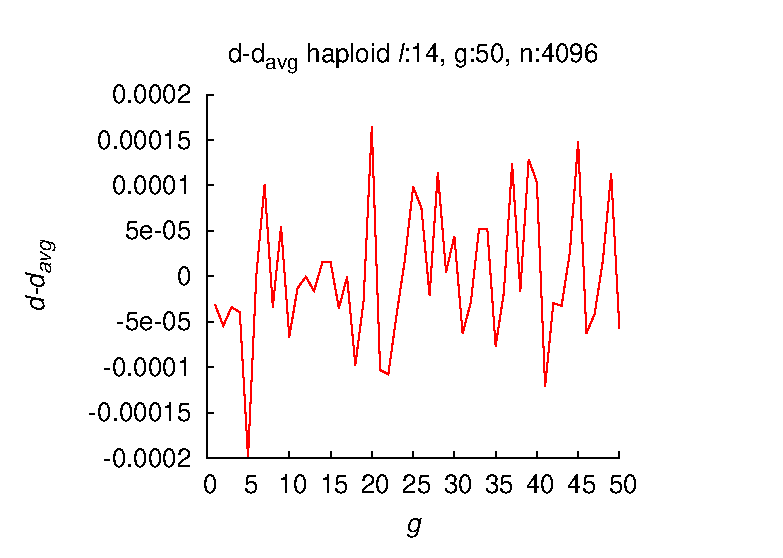
\includegraphics{figures/eps/osc/b14/n004096_osc_fin_hap_dist.eps}}} \vspace{-1em}  \hspace{-3em}% 
\end{center}
\begin{center}
\subfloat{
\resizebox{8cm}{5cm}{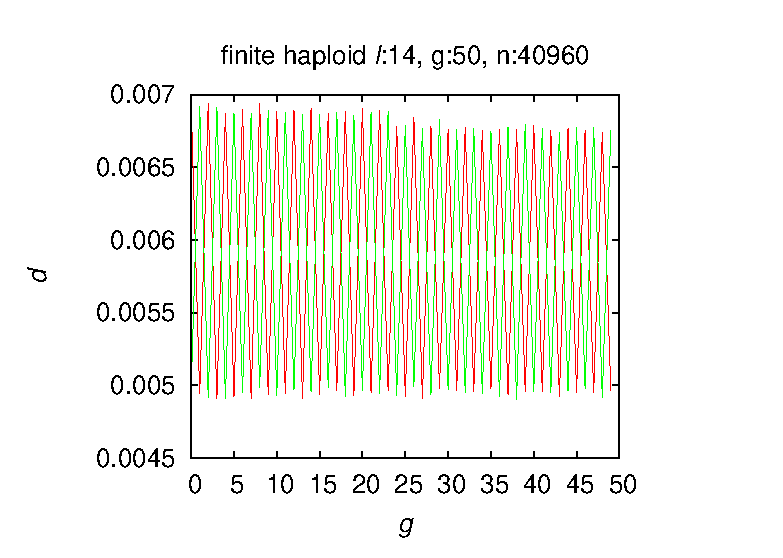
\includegraphics{figures/eps/osc/b14/n040960_osc_fin_hap.eps}}} \hspace{-3em}% 
\subfloat{
\resizebox{8cm}{5cm}{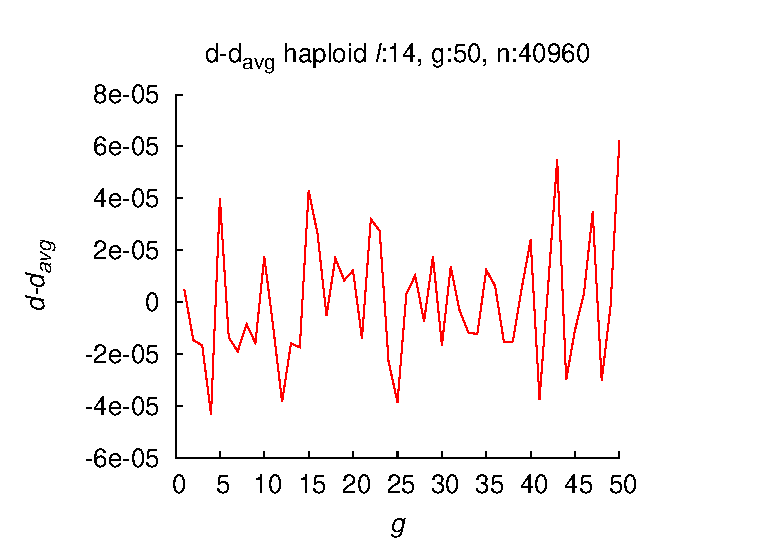
\includegraphics{figures/eps/osc/b14/n040960_osc_fin_hap_dist.eps}}} \vspace{-1em}  \hspace{-3em}% 
\end{center}

\begin{center}
\subfloat{
\resizebox{8cm}{5cm}{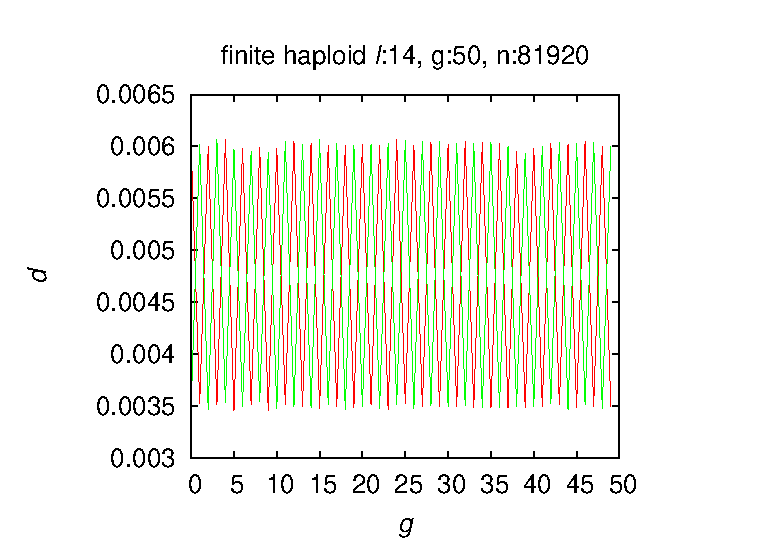
\includegraphics{figures/eps/osc/b14/n081920_osc_fin_hap.eps}}} \hspace{-3em}% 
\subfloat{
\resizebox{8cm}{5cm}{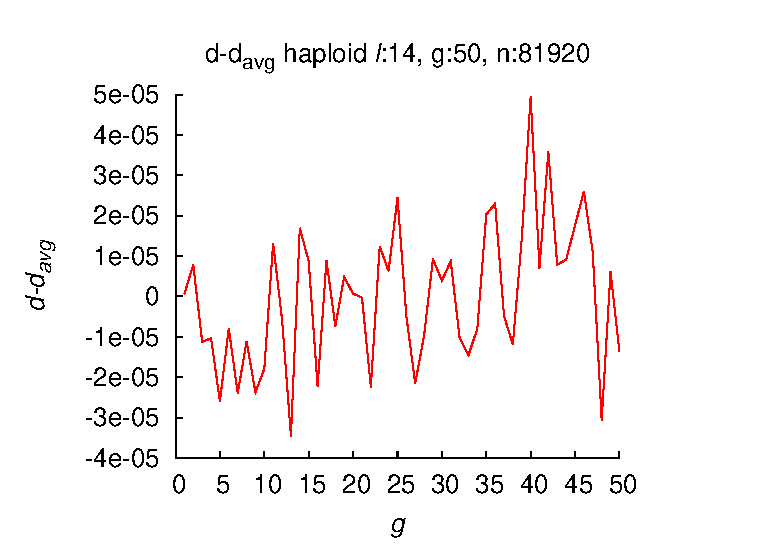
\includegraphics{figures/eps/osc/b14/n081920_osc_fin_hap_dist.eps}}} \vspace{-1em}  \hspace{-3em}% 
\end{center}

\begin{flushleft}
\subfloat{
\resizebox{8cm}{5cm}{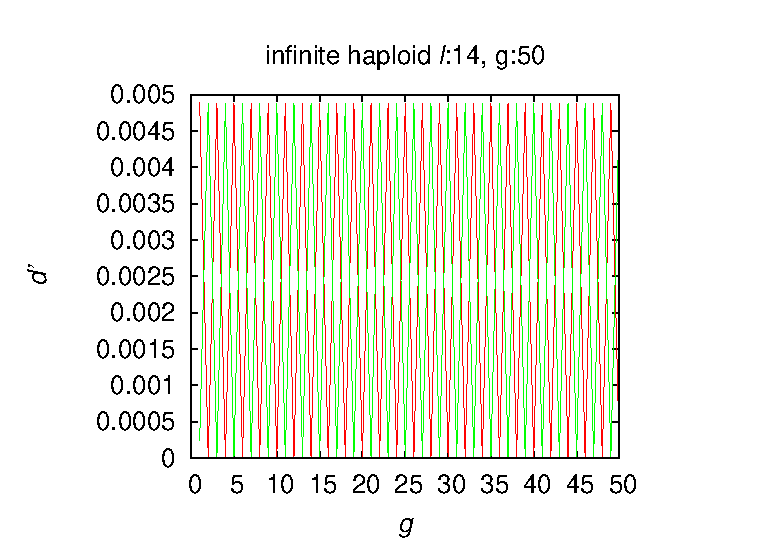
\includegraphics{figures/eps/osc/b14/osc_inf_hap.eps}}} \vspace{-0.5em} \hspace{-3em}%


\caption{\textbf{Infinite and finite haploid population oscillation behavior for genome length $\ell = 14$ (bits):} $d$ is
  distance between infinite or finite population ${\bm q}^n$ and infinite
  population limits ${{\bm p}^\ast}$ and ${{\bm q}^{\ast}}$ for $g$ generations and finite population size $n$.}
\label{oscillation_14h}
\end{flushleft}
\end{figure}

\begin{figure}[H]

\begin{center}
\subfloat{
\resizebox{8cm}{5cm}{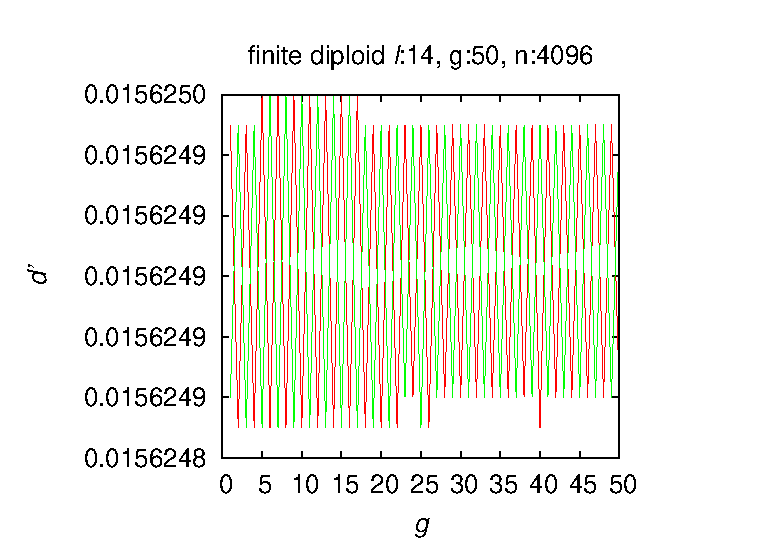
\includegraphics{figures/eps/osc/b14/n004096_osc_fin_dip.eps}}} \hspace{-3em}% 
\subfloat{
\resizebox{8cm}{5cm}{\includegraphics{figures/eps/osc/b14/n004096_osc_fin_dip_dist.eps}}}  \vspace{-1em}  \hspace{-3em}% 
\end{center}
\begin{center}
\subfloat{
\resizebox{8cm}{5cm}{\includegraphics{figures/eps/osc/b14/n040960_osc_fin_dip.eps}}} \hspace{-3em}% 
\subfloat{
\resizebox{8cm}{5cm}{\includegraphics{figures/eps/osc/b14/n040960_osc_fin_dip_dist.eps}}}  \vspace{-1em}  \hspace{-3em}% 
\end{center}

\begin{center}
\subfloat{
\resizebox{8cm}{5cm}{\includegraphics{figures/eps/osc/b14/n081920_osc_fin_dip.eps}}} \hspace{-3em}% 
\subfloat{
\resizebox{8cm}{5cm}{\includegraphics{figures/eps/osc/b14/n081920_osc_fin_dip_dist.eps}}}  \vspace{-1em}  \hspace{-3em}% 
\end{center}

\begin{flushleft}
\subfloat{
\resizebox{8cm}{5cm}{\includegraphics{figures/eps/osc/b14/osc_inf_dip.eps}}} \vspace{-0.5em} \hspace{-3em}%


\caption{\textbf{Infinite and finite diploid population oscillation behavior for genome length $\ell = 14$ (bits):} $d$ is
  distance between infinite or finite population ${\bm q}^n$ and infinite
  population limits ${{\bm p}^\ast}$ and ${{\bm q}^{\ast}}$ for $g$ generations and finite population size $n$.}
\label{oscillation_14d}
\end{flushleft}
\end{figure}
%oscillation